\chapter{Evaluation}
We followed Pol, Koomen and Spillner's way of testing \cite{pol2000management} by using their model and dividing the process of testing into the 
six phases planning, preparation, test-specification, execution and result analysis. Due to extent this work is aimed at, 
it was not feasible to implement all the systems of the related solutions on this field on a common environment
to get a fair assessment for each work and to really estimate how each solution performes against the others. 
On the other hand such a comparison would have to be treated with caution since, each solution is designed with another metric/goal kept in mind.
Si et al. \cite{overview_caa} provide an overview on the current well-known solutions on \ac{CA} and may serve for a further review and comparison.
Therefore the following tests will focus on the comparison between AutoWDS basic and its extended, optimized version.
Furthermore our tests were restricted to the evaluation of spanning tree topolgies, because AutoWDS currently 
still uses a bridged network for its APs instead of a proper routing system, with the drawback of \ac{STP} being active.
\footnote{\ac{STP} is a temporary measure since it does not scale well. 
Our survival paths are supposed to lay the ground for redundancy-systems in layer 2 (like FabricPath \cite{fabricpath}).} 
This means even if we would try to run a network topology with survival paths in it on AutoWDS, \ac{STP} would disable some links in order to 
eliminate circles in the topology \footnote{Circles in a network topology are undesirable since they can lead to broadcast-storms see \ac{IEEE} 802.1D}.
As a consequence achievable throughput will be lower than it could be with survival paths.

\newpage

  \section{Planning}
    The goal of this test is to confirm the claim of an increase in overall throughput of AutoWDS extended compared to AutoWDS basic.
    Therefore we will evaluate the whole process by deploying an actual \ac{WDS} with AutoWDS instead of just performing a code analysis or review.
    To discern performance gains we run AutoWDS basic and extended on the same networking setup and measure its achieving overall throughput.
    In order to create enough throughput we attach traffic generators to the APs to simulate real clients.
    These generators will then send data to all the other nodes in the network.
    To get the values of how much data was actually carried over the wireless network, we will query the APs for this information in a way that it 
    does not affect the measurement, like querying too often for too much data would cause additional load on the APs and the network as a whole.
    
    The scope of the test is kept to the same scale as portrayed in the requirements analysis.
    That means it will not exceed 100 APs with expected target size of about 30 devices.
    We would expect to recognise noticeable differences between the two systems, since interference was strongly avoided where possible and radio modules 
    are more efficiently used than before.
    
    We would expect a significant increase of data that has been able to transmit due to the usage of multiple collision domains, the same one could
    expect by comparing a network hub, which has essentially just one collision domain and a network switch which has multiple domains and does not have
    to wait until the medium is free for sending again. The second source for an increased throughput would be the increased number of packets that could be received
    without errors due to a lessened interference.
    
    \begin{figure}[h!]
      \centerline{
	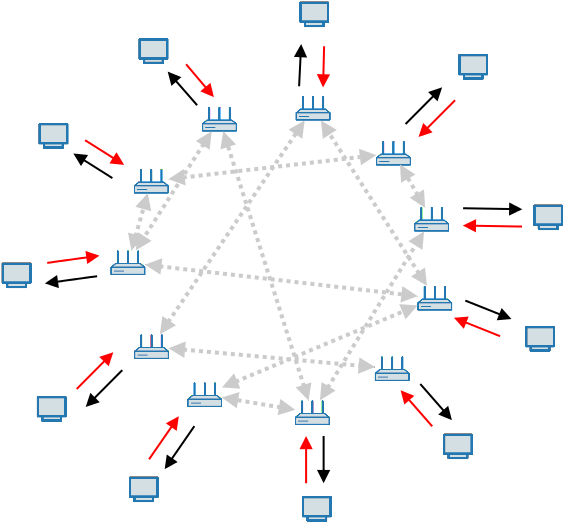
\includegraphics[width=0.6\textwidth]{figures/testsetup_logic}
	\caption{Concept of testbed with traffic-generating systems attached to APs by cable, sending broadcast traffic and saturating the network.}
      }
      \label{fig:testsetup_logic}
    \end{figure}    
    
  \section{Preparation}
    The basic approach for measuring the throughput is to attach traffic generators to the APs and make those send as much broadcast traffic to all
    other stations which are part of this network and therefore saturate the throughput capabilities of the network. 
    The idea behind this setup is to simulate real end-device-clients attached to the APs, where each client has its own ip address and 
    therefore mac- address and table. Cabling the clients to the \ac{AP} instead of using real mobile devices like smartphones was preferred as this gave
    us more control to keep out other impacting effects and moving around 3 Devices per \ac{AP} would have been a challenge, especially to do it in the same
    way for each test-run to keep circumstances reproducible.
    
    Due to limitations in cabling for power and network and severe interference in 
    certain parts of our building we could not use the full 30 APs as initially planned.
    Therefore we had to consider ourselves satisfied with just 12 APs.
    
    \subsection{Modifications for Practical Testing}
      Although we did not have to modify the code of our algorithms for the network, we had to modify the \ac{LCOS} firmware to better fit the 
      data we needed as input for the algorithms to our requirements. Therefore we took the latest stable firmware version 9.0 and added the following extension:
      \begin{description}
	\item[Addition of the Seen-Table:]
	  Although most of the data we needed did already exist in the current \ac{LCOS}-firmware, it was spread over numerous places and retrieving the necessary dates
	  was tedious and performance-costly. That is why we decided to gather everything necessary in one special table (see figure \ref{tab:wlc}).
	\item[Reduced Beacon Rate:]
	  Due to the close proximity of the APs in our testbed we had to reduce the amount of beacons which were sent by the APs to decrease their influence in 
	  the throughput performance test. The default rate with one beacon per 100ms was especially for the mono-channel setup too much as those beacons were received
	  by all 12 other APs. The beacon rate for the test-setup was therefore increased to one beacon per 800ms.
	\item[Default Point-to-Point-Scanning Mode Deactivated:]
	  Per default the APs on a regular basis switch into a scanning mode, where they iterate over all available channels in miliseconds and listen for
	  other radios. During this timeframe the AP can not receive or transmit any data, which would have a drastic dramatic impact on the throughput-tests.
	  This is why we deactivated the scanning mode for the duration of the throughput-test, after the network topology has reached a stable state.
      \end{description}
   
\newpage
   
    \subsection{Physical Structure}
      We deployed the APs at a typical office environment as depicted in figure \ref{fig:2ndfloor} and used only omnidirectional antennas for the APs.
      Additionally the APs were also connected by wire to their client systems on a central server in form of virtual machines.
      
      \begin{figure}[h!]
	\centering
	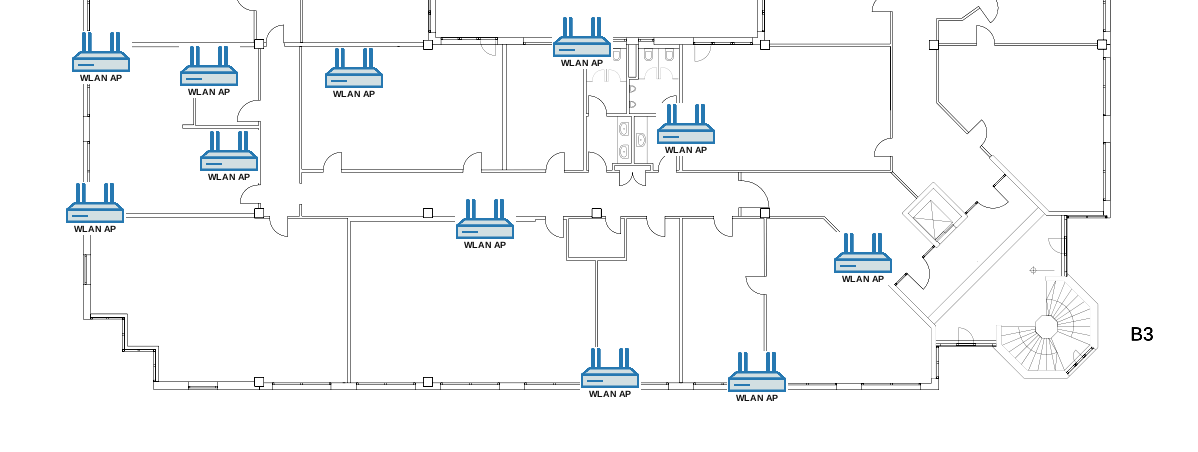
\includegraphics[width=\columnwidth]{figures/Lancom-flur-withaps}
	\caption{Physical arrangement of APs in a typical office complex spread over an area of rougly 15m x 40m}
	\label{fig:2ndfloor}
      \end{figure}
      
      The hardware we used were mainly LANCOM devices and also 6 OpenBAT devices, although flashed with the same firmware.
     
      List of used hardware:
      \begin{itemize}
	\item 3 x LANCOM L-322agn dual Wireless \cite{lancom}
	\item 3 x LANCOM L-452agn dual Wireless
	\item 6 x Hirschmann OpenBAT-R
	\item 1 x LANCOM WLC-4100
	\item 2 x LANCOM GS-2352P
      \end{itemize}
      
      Note that the distance between the APs should have been increased even further to more closely resemble a real usecase-deployment.
      Thus the actual interference would have gone up, since with a lower \ac{SNR} the APs would not have been able to recognize each others 
      transmissions as those and categorize it as interference instead of applying CSMA/CD, leading to more corrupt packets.
      We were able to simulate this problem with a reduced transmit-power to some degree,
      but even on the lowest setting most of the APs were still able to receive each others beacons well enough. 
      This is another factor that will lower general throughput for all setups, which we will notice in the testresults.
      Therefore the throughput-differences between the two systems in a real deployment will probably be higher, since AutoWDS basic will suffer worse from this effect 
      compared to AutoWDS extended.
    
    \subsection{Logical Structure}
      We simulated the traffic generating systems with OpenVZ \cite{openvz} on one server with a \ac{VLAN} for each system to separate the traffic for each client.
      This was done so that we did not need to setup twelve different real hardware machines as those merely have to send and receive traffic.
      The \ac{VLAN} infrastructure is transparent to the VZ containers and the APs, since the host-machine on the server 
      encapsulates all frames before sending it over the \ac{VLAN} Trunk to the switch, which again decapsulates the frames before sending them to the APs.
      
      \begin{figure}[h!]
	\centerline{
	  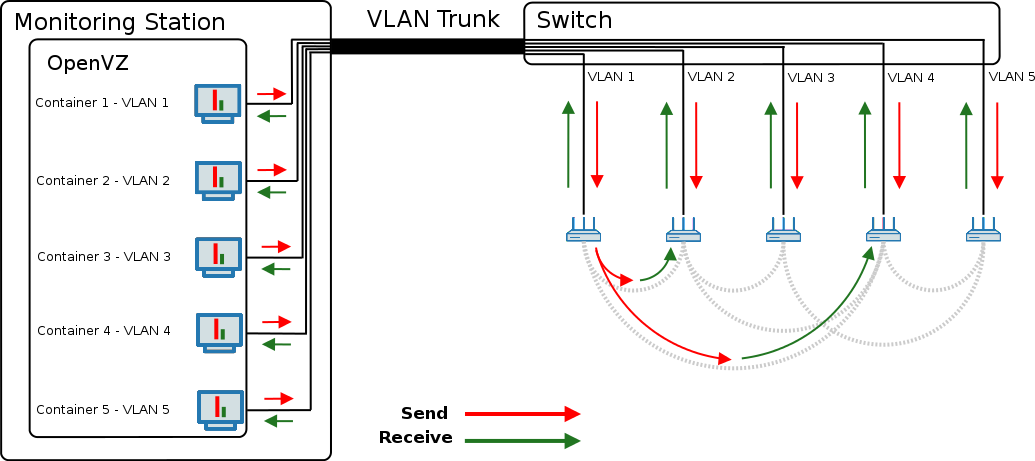
\includegraphics[width=1\textwidth]{figures/testsetup_openvz}%
	  \caption{Test arrangement with OpenVZ and VLANs to simulate a busy network.}
	}
	\label{fig:testsetup_openvz}
      \end{figure}
      
      To generate the traffic we used IPerf \cite{iperf} on the attached systems in \ac{UDP} mode with a datarate of 1Mbit per second for a total of 10 minutes.
      Since we could not directly send \ac{UDP} frames to broadcast addresses with iperf, we ran multiple instances of iperf with different target ip addresses.
      Although 1Mbit for each stream may not seem much, but after multiplying it with the number of targets and the up- and downstreams the effective rate results in
      1Mbit * 12 * 2 = 24Mbit/s for each \ac{AP}. As we will see later on, this will turn out to be enough to entirely saturate the wireless network but is still within
      the capabilities of the used Gigabit Ethernet to get the data to and from the APs, 
      as 24Mbit/s * 11 = 264Mbit/s does not exceed the 1000Mbit/s \ac{VLAN} Trunk connection as possible bottleneck.
      
      \begin{listing}[h!]
	\begin{lstlisting}
iperf -u -c 172.16.40.2* -t 600 -b 1M
	\end{lstlisting}
	\caption{IPerf mode of operation for generating the traffic.}
	\label{lst:iperf}
      \end{listing}
    
\newpage
    
  \section{Specification}
    Each test run describes a 10 minutes performance stress test for the network with throughput saturation. 
    This should be enough time to notice any temporal effects and to get a picture of the lasting performance.
    
    To keep environmental conditions for each of the AutoWDS systems as similar as possible we conducted the runs alternatively with respect to channel usage.
    So that a possible temporal interference in a certain band would affect both runs and not just favor a single system.
  
    Actually to get more statistic significance we should have run this test-array more than once, but as for each new setup there had to 
    be invested a considerable amount of time in the pre-setup of AutoWDS (getting it up and running, despite bugs), 
    this was not feasible within the timeframe that was scheduled to execute the whole evaluation.
    
    Additionally we ran the testcases with two different antenna power-settings to simulate the hidden station problem. 
    Therefore we first set the radios to full power resulting in a high connectivity between the nodes and on a second 
    run decreased the transmit power as much as possbile to get a network with a smaller degree of interconnectivity.
  
    \begin{table}[h!]
      \centering
      \begin{tabular}{clll}
	Testrun nr. & AutoWDS version & Channels used & Antenna power\\ \hline
	1 & basic & 1 & low \\
	2 & extended & 1,6,11 & low \\
	3 & basic & 36 & low \\
	4 & extended & 36,40,44 & low \\
	5 & basic & 1 & high \\
	6 & extended & 1,6,11 & high \\
	7 & basic & 36 & high \\
	8 & extended & 36,40,44 & high \\
	9 & extended & 1,6,11,36,40,44 & low \\
	10 & extended & 1,6,11,36,40,44 & high \\
      \end{tabular}
      \caption{Testruns executed with different channelusage and varying antenna power.}
      \label{tab:testruns}
    \end{table}
    
\newpage
    
  \section{Execution}
    The tests were executed mainly in the evening and on weekends in order to catch those short timeframes where the radio bands are not as crowded as on ordinary workdays.
    The general procedure for a testrun was implemented as follows:
    \begin{enumerate}
      \item Power on the System (\ac{WLC} + APs).
      \item Wait until all APs are connected to the wireless backbone (see description of AutoWDS in chapter \ref{autowdsbasic}).
      \item For AutoWDS basic we continue with the next step, for the extended version also the following additional steps have to be conducted.
	\begin{enumerate}
	 \item Wait until all the wireless measurements arrived at the \ac{WLC}.
	 \item Run our algorithm, which reads data from the \ac{WLC}, computes a solution and writes back the topology-to-do to the \ac{WLC}.
	 \item Wait until the \ac{WLC} reconfigured all the APs.
	 \item Wait until the APs all successfully reconnected through their new connections to the wireless backbone.
	\end{enumerate}
      \item Start the scripts that iteratively query the APs for their status tables every 7 seconds \footnote{Seven seconds is roughly as long as it took the testcore
      framework to query the APs for all their table-data. Querying them more often would have had an impact on their performance.}
      \item Start the receiving iperf processes on the VZ machines.
      \item Start the sending iperf processes on the VZ machines.
      \item Wait the predefined 10 minutes until the tests finish.
      \item Archive the collected data.
    \end{enumerate}
    
\newpage

    During the testruns we made snapshots of the network topolgies, where you can actually see the improvements.    
    \begin{figure}[h!]
      \centering
	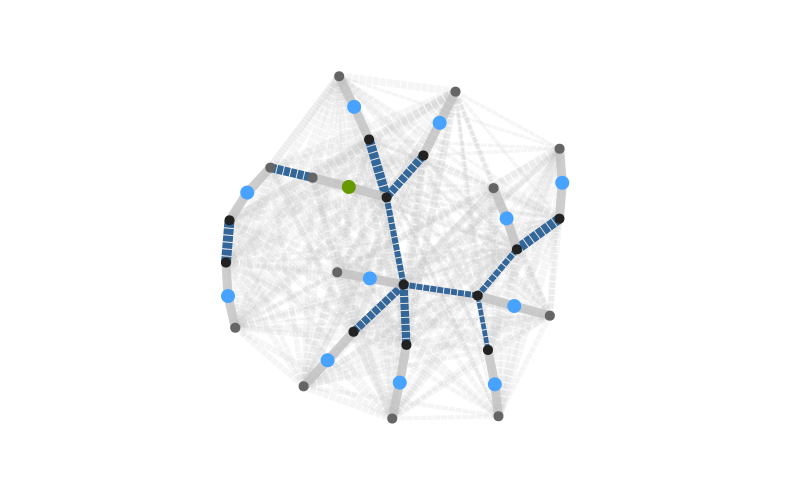
\includegraphics[width=\textwidth]{figures/topo_chan_1}
	\caption{Topology of the testnetwork with only one channel in use (AutoWDS basic).\protect\footnotemark }
      \label{fig:topo_chan_1}
    \end{figure}
    
    \footnotetext{Different edge-colors indicate different channels. Also edge thickness denotes the quality of a link, where thicker means higher quality.}

    \begin{figure}[h!]
      \centerline{
	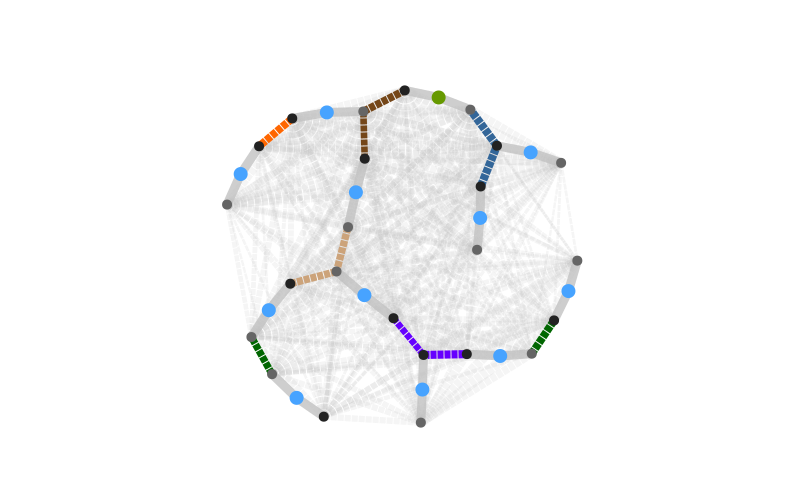
\includegraphics[width=\textwidth]{figures/topo_chan_1_6_11_36_40_44}
	\caption{Topology of the testnetwork with six channels in use (AutoWDS extended).}
      }
      \label{fig:topo_chan_1_6_11_36_40_44}
    \end{figure}
    
\newpage
    
    After gathering and aggregating all the archived data from the testruns, we receive the following performance charts.
    
    \begin{figure}[h!]
      \centerline{
	\includegraphics[width=0.62\textwidth]{figures/TestDataDiagramme/20/rx_bytes}%
	\includegraphics[width=0.38\textwidth]{figures/TestDataDiagramme/20/rx_bytes_boxplot}%
      }
      \caption{Received bytes with decreased antenna transmit power}
      \label{fig:rx20_bytes}
    \end{figure}
    
    \begin{figure}[h!]
      \centerline{
	\includegraphics[width=0.62\textwidth]{figures/TestDataDiagramme/3/rx_bytes}%
	\includegraphics[width=0.38\textwidth]{figures/TestDataDiagramme/3/rx_bytes_boxplot}%
      }
      \caption{Received bytes with full transmit power}
      \label{fig:rx3_bytes}
    \end{figure}
    
    Analyzing the successfully received bytes for the low power (figure \ref{fig:rx20_bytes}) and high power (figure \ref{fig:rx3_bytes})
    setup we recognize noticeable differences for each channel-assignng.
    
      \begin{itemize}
	\item The base scenarios where only one channel was utilized performe the worst within a range of 0.5 to 1.5Mbit/s on average per \ac{AP}.
	  Using three channels gives roughly three times the throughput (2.5 - 5Mbit/s for 2.4 GHz and 2.5 - 5Mbit/s for 5 GHz) compared to the baseline.
	  Utilizing up to 6 Channels shows the best results with an effective throughput of 5.5 - 9Mbit/s. Note that the gain for the 6 channel setup 
	  is still linear as it provides roughly 6 times the throughput of the baseline.
	\item We further discern that the high transmit power setup outperformes the low power setup by a factor of two with an even more noticeable difference.
	\item With slight variations for the high-power 3/2.4 GHz setup the rates are also rather constant.
	\item Besides the high-power 1/5Ghz setup we realize 5 GHz's superiority over the 2.4 GHz band.
      \end{itemize}

    \begin{figure}[h!]
      \centerline{
	\includegraphics[width=0.56\textwidth]{figures/TestDataDiagramme/3/recpackerr}
	\includegraphics[width=0.44\textwidth]{figures/TestDataDiagramme/3/recpackerr_boxplot}
	\caption{Ratio of successfully received packets to packets containing errors for reduced transmit power scenario}
      }
      \label{fig:3recpackerr}
    \end{figure}
    \begin{figure}[h!]
      \centerline{
	\includegraphics[width=0.56\textwidth]{figures/TestDataDiagramme/20/recpackerr}
	\includegraphics[width=0.44\textwidth]{figures/TestDataDiagramme/20/recpackerr_boxplot}
	\caption{Ratio of successfully received packets to packets containing errors for full transmit power scenario}
      }
      \label{fig:20recpackerr}
    \end{figure}
    
\newpage
    
    From the existing data we could also extract the number of errors over time. Deriving the rates and setting those in proportion to
    successfully and all transmitted packets we can now take a look at the effective rate of corrupt packets and therefore bytes, 
    as an error in a packet spoils the whole packet and all data in it.
    \begin{itemize}
      \item The base-scenario again performs subpar and shows the highest error rates with 10 to 65 percent depending on the transmit power.
	Using three channels, the error-rates shrink down to 6 to 30 percent.
	Adding another three channels seems to further reduce error rates to 5 to maximal 10 percent.
      \item As with the successfully transmitted bytes we note a greater difference when using different transmit power setups. 
	Increasing the transmission power also increases the error-rates at least twice and up to 6 times (one channel/ 2.4 GHz).
      \item In the low-power setup error-rates are rather constant compared to the high-power setup where 
	we discern greater deviations especially for those tests in the 5 GHz band.
    \end{itemize}
    
    Note that different from Pol, Koomen and Spillner's recommendation \cite{pol2000management} the test was not run by someone impartial, but also by us.

  \section{Analysis}
    The results match our expectations, despite all the limitations of our testbed.
    Using only a single channel in AutoWDS basic does not scale well, no matter how much transmit power is used and independent of the band.
    Not only is the baseline scenario incapable of transmitting much data, most of it is also corrupt.
    The results also affirm our estimate that the basic version transfers only a little more than control data.
    
    While setting up the test environment we also noticed that this effect of medium overload is no result of the size of our network.
    Whereas two unimpeded APs were able to achieve a throughput of about 2Mbit in each direction, adding a third one would dramatically 
    decrease overall throughput down to about 100kbit or less, growing worse with each newly added \ac{AP} in receive-range. 
    Even spreading the APs further apart would not promise better results since the inherent problem of reusing the same channel for the forwarding and receiving 
    link restricts the forwarding capabilities drastically.
     
    As the figures show, the outcome is dependent on the number of channels used as a setup with only three distinct channels allowed yields still better
    results than a mono-channel-setup but is inferior to a setup where we can use even more channels as this gives us the possibility to use more collision domains
    which results in more available bandwidth and therefore increased throughput. In our example we used APs with only two radios, which
    limits us in selecting separate modules for different connections so that an \ac{AP} which already established two connections over its two modules
    would have to share one of its modules in order to apply a new link to a foreign Ap in order to maintain connectivity.
    This means instead of just using a lot of channels or just using a lot of radios per \ac{AP} a combination of both promises the best results.
    \begin{figure}[h!]
      \centerline{
	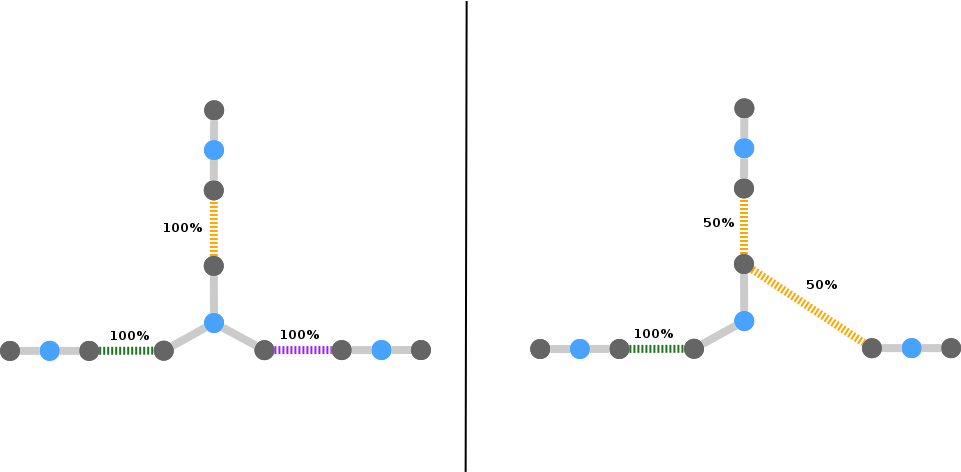
\includegraphics[width=\textwidth]{figures/3modulesvs2}
	\caption{Link separation capability for an \ac{AP} with three modules compared to an \ac{AP} with two modules.}
      }
      \label{fig:3modulesvs2}
    \end{figure}
    
    Compared to the base scenario our link selection and channel assignment algorithm roughly doubles the throughput with every channel added. 
    Of course this effect is limited by using a separate channel for each link and also by the number of modules for an \ac{AP} 
    since the former effectively assigns each link its own channel and the latter is a question of practical relevance as current APs are only 
    shipped with two or a maximum of three radio modules. As our gathered data indicate, it is after all a notable improvement to utilize multiple channels and modules.
    
    \subsection{Reflection on the Requirements}
      In this section we will analyze by how far we were able to meet the imposed requirements and restrictions from the requirement analysis.
  
      \begin{description}
	\item [Increased Throughput:]
	  Our measurement results indicate that throughput could considerably be increased. How much is determined by the input parameters of the algorithms like
	  channels that can be utilized and hardware environments like the number of radio modules available at the APs. 
	  
	\item[Reduced end-to-end Link Failures:]
	  The survival path property takes care of this requirement. That is for the given error-scenario of one failing connection at a time, there is always
	  a backup connection over a different link available as far as the underlying topology permits. We were not able to test this feature 
	  with the given implementation, but we are nevertheless confident that also this requirement has been met. 
	  At least in theory it fulfills the 2-edge-connectedness attribute in the resulting graph.
	  If multi-flow / routing support will be implemented for our hardware in the future, a decrease in node separation for failing links should be recognizable.
	  
	\item[Multiple Radios Utilized:]
	  Our algorithm utilizes the radio-modules as far as they are relevant for creating links between APs with a high estimated throughput.
	  Depending on the given infrastructure not all radio modules are necessarily used, since not all of them are needed in order to create a connected network topology.
	  Moreover using all available links may not necessarily be beneficial, since if not enough radios are available, adding new links can force
	  other radios to the same channel, which effectively leads to sharing a single channel between more radios instead of exclusive access (see figure \ref{fig:lessismore}).
	  
	  Having some radio modules to spare gives us the opportunity to use those exclusively for client 
	  connections and assigning them a channel which does not interfere with the wireless backbone.
	  
	  \begin{figure}[h!]
	    \centerline{
	      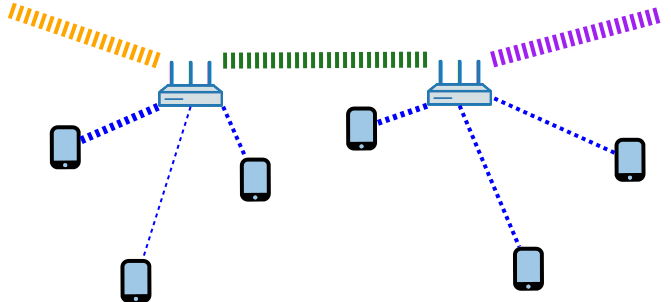
\includegraphics[width=0.56\textwidth]{figures/moduletospare}
	      \caption{Unused modules can be used for separate client connections without interfering the \ac{WLAN} backbone. 
	      This setup would require at least three radios on each \ac{AP}.}
	    }
	    \label{fig:moduletospare}
	  \end{figure}
	
	\item[Capability of Using Variable Channelsets:]
	  Our algorithm selects channels from a given input set of channels. Only those channels are then used to determine the channel assignment.
	  It is even possible to specify only one channel, resulting in a topology optimized network graph only.
	  Therefore this solution also fullfills this requirement.  
	  
	\item[Centralized Computation and Configuration:]
	  The requirement dictates that computing a solution should be possible on a centralized entity (servers / \ac{WLC}).
	  Our algorithm was implemented as a python script and can be run on a single system if given the right input data.
	  Creating the configurations for the \ac{AP} will still be conducted by the central WLC as depicted in \ref{fig:dataflow}.
	  
	\item[Static Environment:]
	  Also the second requirement is taken into consideration, since our algorithm is specially designed for a static environment where link quality 
	  and linkstate stay the same for a foreseeable time.
	  If major changes in network connectivity or link quality occur, the chosen network topology and channel assignment
	  may lead to temporal suboptimal results, therefore also a recomputation of the network topology would have to be triggered.
	  Currently there are no automatic triggers implemented, so that an administrator would have to decide when to optimize the network (commonly after initial deployment),
	  but our algorithm can be further extended for an automatic self-optimizing network.
	  
	\item[Layer 2 Usage:]
	  APs still use bridged point to point connections after our optimization to span the wireless network backbone, therefore creating no obstacles for Layer 2 frames.
	  The ethernet frames are just forwarded like in a switched environment and are not encapsulated in layer three packets.
	  The survival paths pave the way for different routing systems, yet still to come. Eventual systems include FabicPath \cite{fabricpath}, \ac{MPLS} \cite{mpls} and 
	  Layer 3 routing only (breaking the Layer 2 connectivity).
	  
	\item[Economic Constraints:]
	  Algorithm runtime mainly depends on the number of connections between the nodes. Calculating the initial spanning tree is done in \ac{BFS} mode and 
	  therefore has quadratic runtime for the worst case, depending on how sparse the graph is. The following calculation of the survival paths has also quadratic runtime 
	  since we iterate over all connections and for each connection in the worst case over all other connections to find the backup path.
	  In a common deployment scenario the underlying network graph will be rather sparsly connected since the number of APs used and placement are carefully selected.
	  Typically they are placed in a way that they span a network over an area as far as possible.
	  Current deployments and deployments in near future won't exceed 100 APs. 
	  Even if fully meshed with a total of \(\sum \limits_{i=1}^{100} i = \frac{100(100+1)}{2}=5050\)
	  edges it won't pose a problem to the capabilities of a \ac{WLC} or an administrators machine.
	  
      \end{description}
      
\newpage
      
    \subsection{Reflection on Related Work}
      Comparing our solution to those of others would need a common ground. 
      For example hardware requirements, number of modules and in general heterogenity / homgenity of
      the network are factor that could play in favor of some algorithms and therefore won't lead to fair results. 
      Additionally different solutions were designed to achieve different goals like throughput, latency or weighted throughput networks. 
      Certainly we could agree on this common deployment and compare each solution for random networks with respect to throughput, 
      but this would require a full-scale simulation as hardware-resources are limited and too easily prone to real world difficulties.
      Although maybe a key aspect, we did not have enough time to simulate even our own solution to the full extent and therefore neither those of others. 
      Nevertheless we would appreciate further work on this approach. 
      In order to at least provide some kind of comparison we will take a look at the features of our work, which most of the related work did not show or provide.
      
      \begin{description}
	\item [Variable Nr. of Radios:] Our algorithms support a variable number of radios on each device instead of a fixed numer like in \ac{INSTC} \cite{INSTC}. 
	  This allows to optimize the wireless network even for heterogeneous environments where devices have a variable number of radios or just simply one.
	\item [Vendor Neutral:] Although we used only LANCOM devices in our case, the solution is vendor neutral. As long as the devices provide the required data,
	  any network with devices that can be configured (also manually) to use a specific link for a certain radio can profit from our optimization.
	\item [No MAC changes:] Our solution does not require any \ac{MAC}-layer changes and can be run on any commodity \ac{WLAN} hardware.
	\item [No Forced Backup Links:] Thanks to our modular approach, adding redundant links to the initial \ac{MST} is optional. 
	  You are free to only optimize and use the \ac{MST} if you are also limited by the \ac{STP}, like we were in our evaluation.
	\item [Considers Foreign Interference:] Admittedly we are not the first to do so (\ac{BFS-CA} \cite{BFS-CA}), but our solution also 
	  considers foreign interfering WLANs which can have a great impact in performance if neglected.
	\item [Customizable Survival Pats:] In order to create the redundant links (survival paths) we iterate over each link in the \ac{MST} and simulate it failing.
	  You could just as well iterate over the nodes in the \ac{MST} to get a \textit{k}-node-connected survival graph or whatever order you chose.
	  This means you can add redundant links in decreasing order of optimality up to a fully meshed graph.
	\item [Customizable Ranking-Formula:] Without great effort you can also adapt the ranking-formula and create a spanning tree which is optimal to some other metrics you need.
	\item [No Gateway/Special Node necessary:] At last you do not need a special gateway node like in \ac{BFS-CA} \cite{BFS-CA} to start our algorithm with.
	  This is especially usefull in setups where all the node are equal or a uplink to the internet is not desired.
      \end{description}